\documentclass{beamer}
\usepackage{graphicx}
\usepackage{tikz}
\usetikzlibrary{shapes,arrows}
\usepackage{tikz}
%\usecolortheme{seahorse}
  \setbeamertemplate{footline}[page number]
\usepackage{multirow}
\setbeamertemplate{navigation symbols}{}
\setbeamertemplate{frametitle}[default][center]
\setbeamerfont{frametitle}{shape=\scshape}
\usepackage{color}

\usepackage{csquotes}

\usepackage{xcolor}

\usepackage[flushleft]{threeparttable}

{\title{\textsc{Econ 352 - Inflation: Phillips Curves and Neo-Fisherism} \\ \tiny (See Williamson Ch. 15)}
\author{Trevor S. Gallen}
\date{}
\begin{document}
\renewcommand*{\inserttotalframenumber}{\pageref{lastframe}}


\setbeamertemplate{caption}{\raggedright\insertcaption\par}

\begin{frame}
\titlepage
\end{frame}

\begin{frame}
\frametitle[alignment=center]{A Warning}
\begin{itemize}
\item A warning: there is a school of thought that takes the New Keynesian model and thinks about its implications seriously
\bigskip
\item Stephen Williamson, the author of our textbook, is one such person!
\bigskip
\item There is a ``curious" or even ``heterodox" conclusion that comes from this orthodox model, which some brand ``Fisherian" or ``Neo-Fisherian"
\bigskip
\item Raising interest rates may \emph{increase, not decrease} inflation
\bigskip
\item Williamson is an outlier, but with good company--I'm more agnostic, but the Fisher relation keeps me up at night
\end{itemize}
\end{frame}

\begin{frame}
\frametitle[alignment=center]{Inflation}
\begin{itemize}
\item Inflation is important!  
\begin{itemize}
\item Hyperinflation is devastating to real production
\bigskip
\item Even moderate amounts of inflation cost ``shoe-leather"
\bigskip
\item Inflation uncertainty affects credit market uncertainty
\bigskip
\item Unexpected inflation has distributional effects
\bigskip
\item In a model with sticky prices, there can be employment/real effects
\end{itemize}
\item So we'll first go through the standard model, then the Neo-Fisherian one
\end{itemize}
\end{frame}


\begin{frame}
\frametitle[alignment=center]{Phillips Curve}
\begin{itemize}
\item We claim that there is a ``Phillips curve," a relation between inflation and output (or unemployment)
\bigskip
\item If inflation from period 0 to 1 is higher than firms expected in period 0, then their prices are artificially low
\bigskip
\item Households will demand more (and firms will produce it, even though prices suboptimally (to them) low, because still making a profit (monopsonistic competition))
\bigskip
\item We write this as:
$$i=a(Y-Y_m)+bi'$$
\item Where $i$ is the inflation rate, $Y$ is GDP, $Y_m$ is the ``efficient" level of GDP, $a>0$, and $0<b<1$.  
\bigskip
\item Idea: the higher inflation, the smaller the ``output gap"
\item Also: higher future inflation, the higher current inflation, as firms that can change prices in anticipation 
\end{itemize}
\end{frame}



\begin{frame}
\frametitle[alignment=center]{Fisher Relation}
\begin{itemize}
\item Fisher relation: the real interest rate is the nominal interest rate minus anticipated future inflation:
$$r=R-i'$$
\item We can use $i=a(Y-Y_m)+bi'$ and the Fisher relation in the NK model to determine inflation (assume i' fixed)
\bigskip
\item Logic:
\begin{enumerate}
\item $R$, the nominal interest rate, is set by the central bank
\item $i'$, inflation expectations, are exogenous/set
\item $R-i'$ affects $Y$ (the ``output demand" curve or the ``IS" curve 
\item $Y$ determines $i$ via $i=a(Y-Y_m)+bi'$
\end{enumerate}
\item Let's see it graphically
\end{itemize}
\end{frame}

\begin{frame}
\frametitle[alignment=center]{The Basic New Keynesian Model}
\begin{figure}
\centering
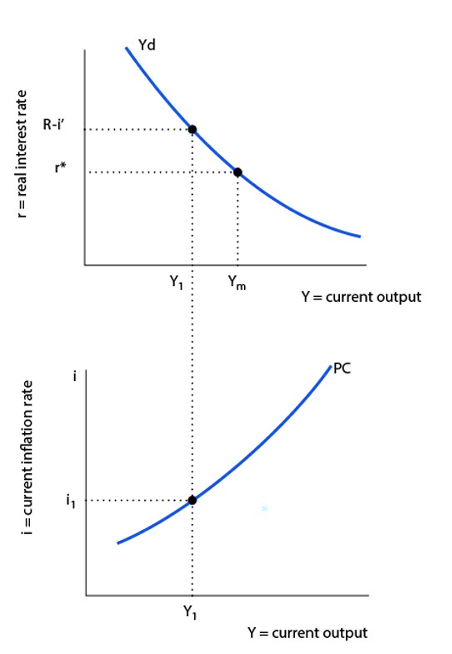
\includegraphics[scale=0.75]{Figures/W_Fig_15pt1.png}
\end{figure}
When $r^*=R-i'$, then $Y=Y_m$, and the economy is ``at capacity"
\end{frame}

\begin{frame}
\frametitle[alignment=center]{Monetary Policy Goals}
\begin{itemize}
\item The logic is that central bank controls $R$, which affects $Y$, which affects $i$
\bigskip
\item How do we determine $R$?  ``optimal monetary policy"
\bigskip
\item Federal Reserve: dual mandate of ``price stability" and ``maximum employment" (tradeoff between $Y$ and $i$)
\bigskip
\item If the real rate of interest $r^*$ decreases, $Y_m$ rises, then how should the bank respond?
\begin{itemize}
\item Could decrease nominal interest rate so $Y'=Y_m'$, but then $i$ would rise
\item Could do nothing, but then output gap (unemployment, for instance) would rise
\item If weights both, then do something in the middle
\end{itemize}
\item Let's see it graphically
\end{itemize}
\end{frame}

\begin{frame}
\frametitle[alignment=center]{The Basic New Keynesian Model}
\begin{figure}
\centering
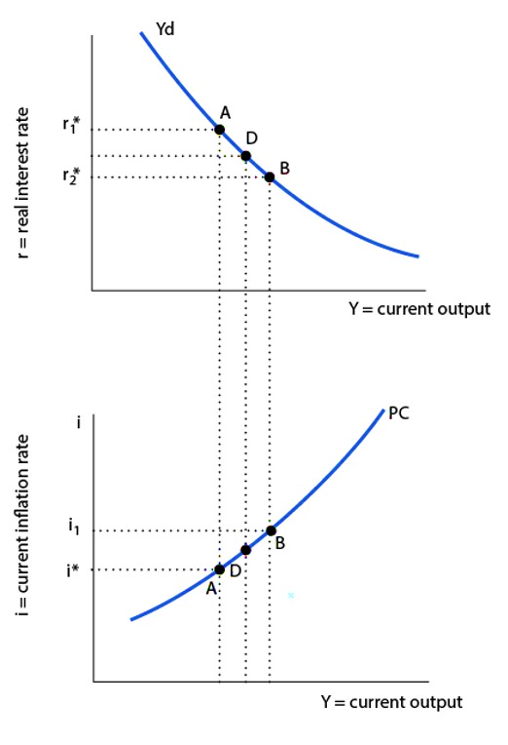
\includegraphics[scale=0.5]{Figures/W_Fig_15pt2.png}
\end{figure}
We start at $A$, but events shift us to $B$, and we split the difference and choose $D$, so output below potential but inflation lower than it would be
\end{frame}


\begin{frame}
\frametitle[alignment=center]{Increase in $i'$}
\begin{itemize}
\item When $i'$ shifts, the ``intercept" of the Phillips curve increases
\bigskip
\item Inflation is now higher than it would be
\bigskip
\item Central bank has a few options
\begin{itemize}
\item Could do nothing: $R+i'$ increases because $i'$ increases, real interest rates increase, output falls, inflation falls
\item Could keep: $R+i'$ constant.  Output doesn't change, but inflation high.
\item Could split the difference, and output falls a little and inflation rises a little.
\end{itemize}
\item Let's see it graphically
\end{itemize}
\end{frame}


\begin{frame}
\frametitle[alignment=center]{The Basic New Keynesian Model}
\begin{figure}
\centering
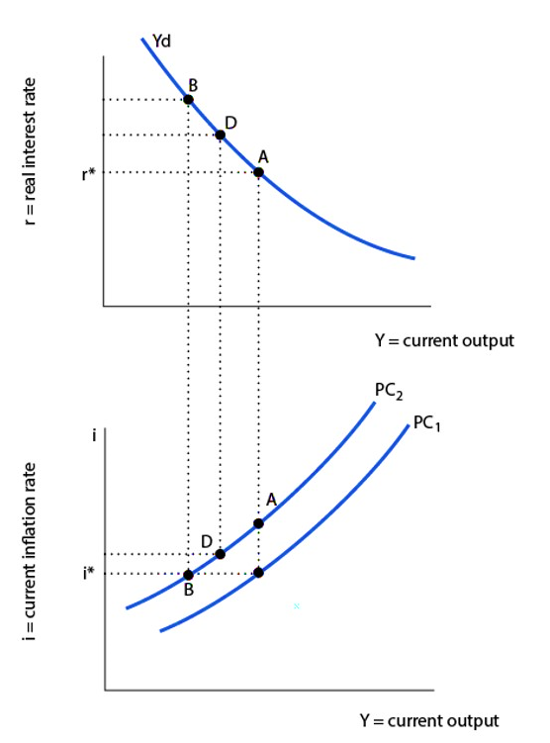
\includegraphics[scale=0.5]{Figures/W_Fig_15pt3.png}
\end{figure}
We start at $A$, but events shift us to $B$, and we split the difference and choose $D$, so output below potential but inflation lower than it would be
\end{frame}


\begin{frame}
\frametitle[alignment=center]{Phillips Curve in the Data}
\begin{figure}
\centering
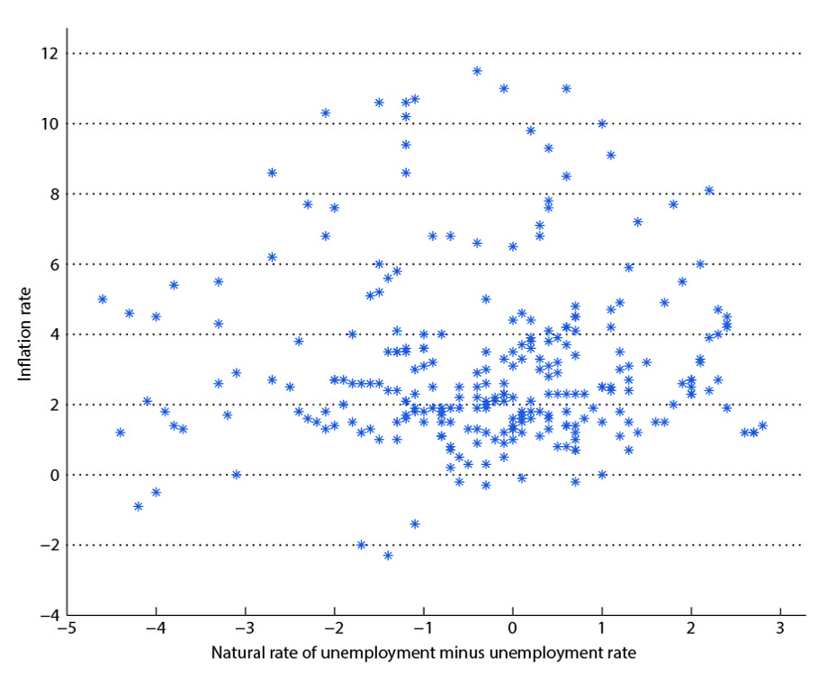
\includegraphics[scale=0.5]{Figures/W_Fig_15pt4.png}
\end{figure}
We assumed a relationship between $i$ and $Y^*$, but it's not so clear that there is one
\end{frame}



\begin{frame}
\frametitle[alignment=center]{Phillips Curve in the Data}
\begin{figure}
\centering
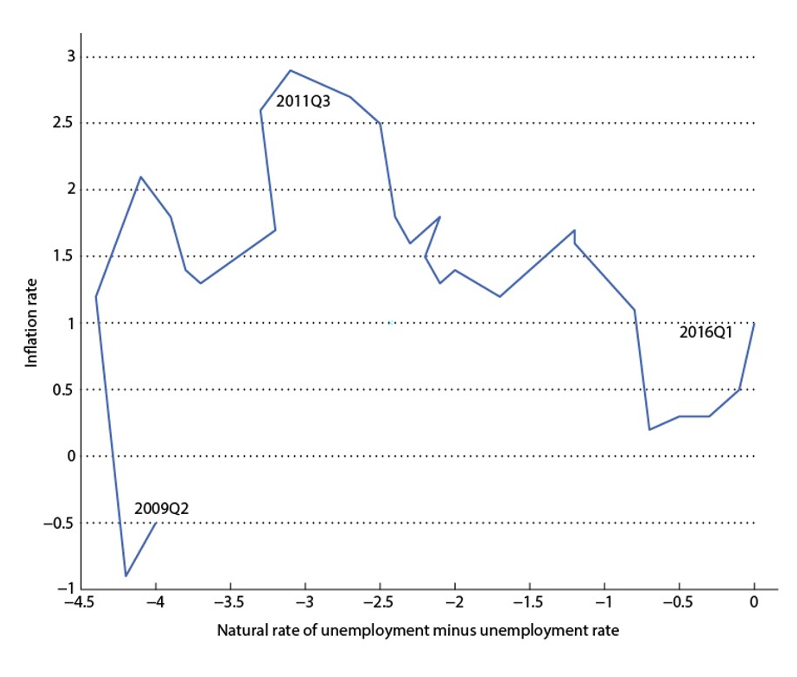
\includegraphics[scale=0.5]{Figures/W_Fig_15pt5.png}
\end{figure}
We assumed a relationship between $i$ and $Y^*$, but it's not so clear that there is one
\end{frame}


\begin{frame}
\frametitle[alignment=center]{Phillips Curve in the Data}
\begin{figure}
\centering
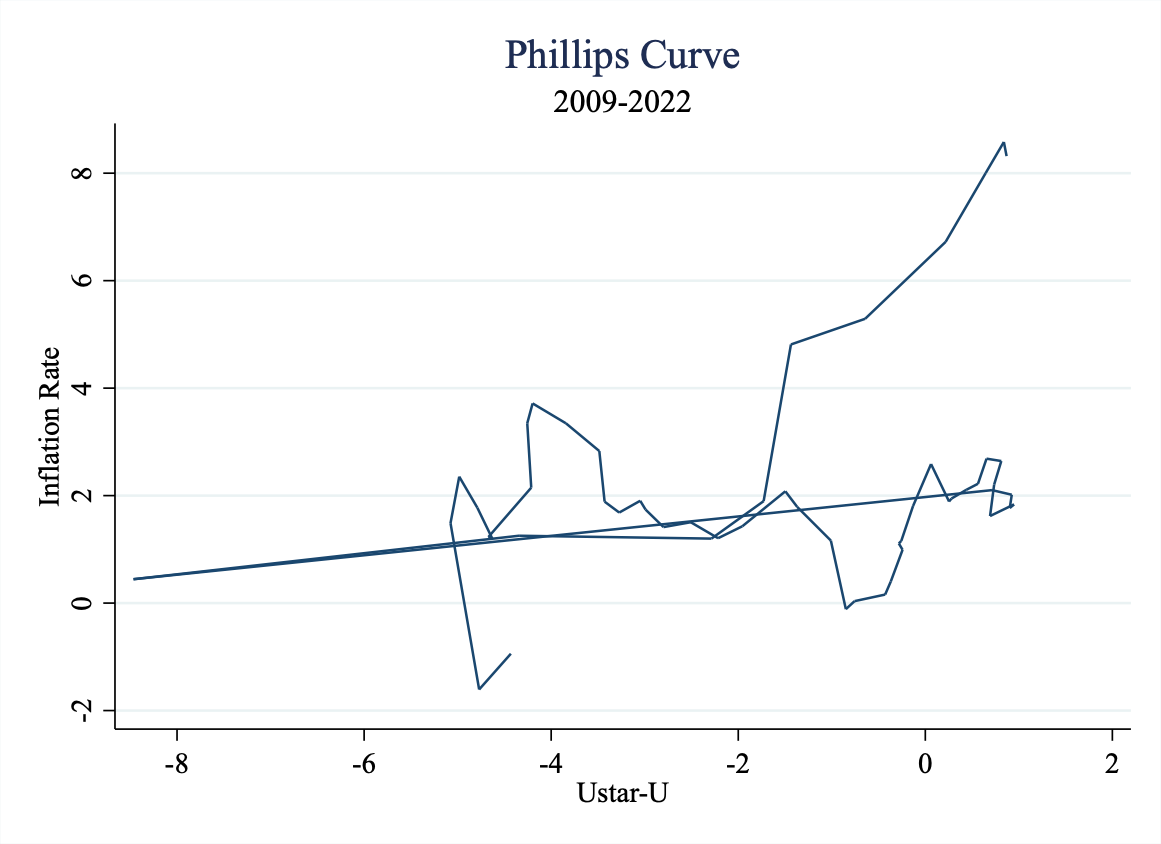
\includegraphics[scale=0.25]{Figures/PhillipsCurve1.png}
\end{figure}
Relationship
\end{frame}

\begin{frame}
\frametitle[alignment=center]{Phillips Curve in the Data}
\begin{figure}
\centering
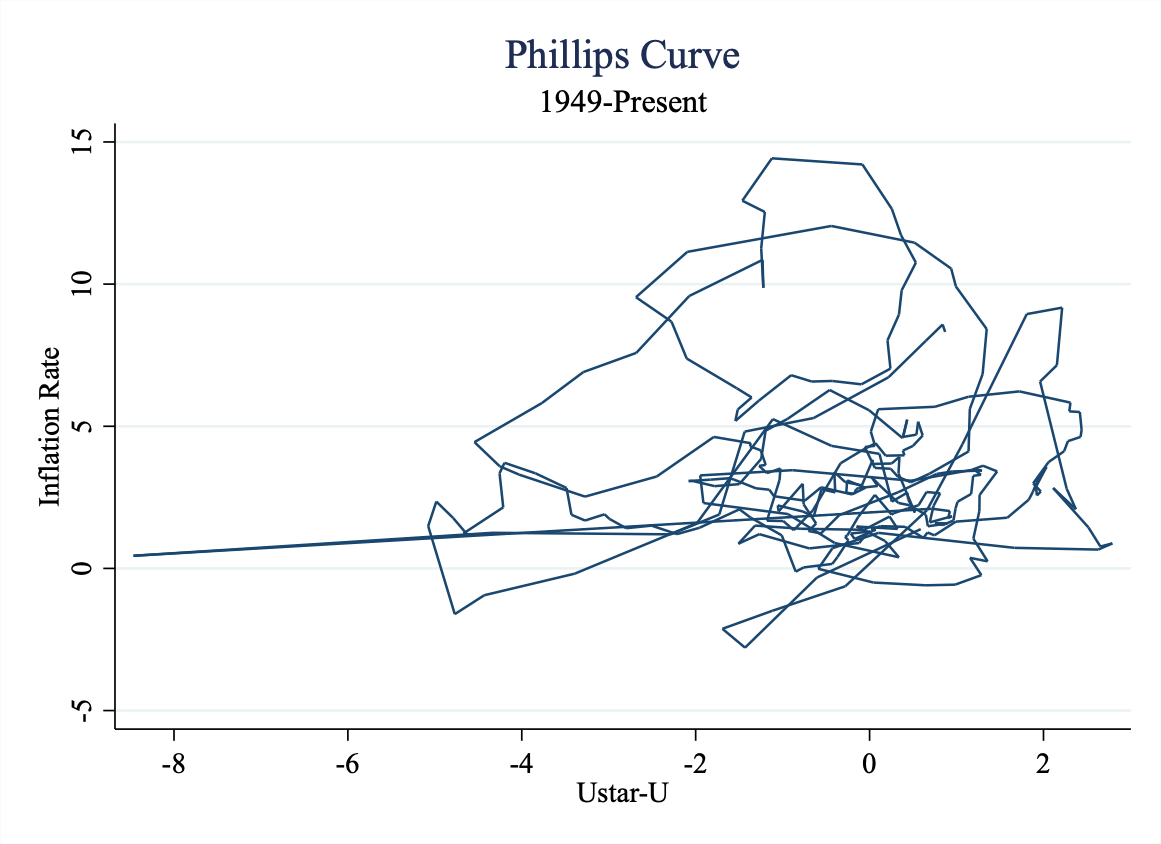
\includegraphics[scale=0.25]{Figures/PhillipsCurve2.png}
\end{figure}
The long view
\end{frame}


\begin{frame}
\frametitle[alignment=center]{Low Real Interest Rates and the ZLB}
\begin{itemize}
\item We now have real interest rates $r$ distinct from nominal interest rates $R$
\bigskip
\item It's been observed that global real interest rates have been falling secularly for some time
\bigskip
\item When $r$ is low, then it's hard for the bank to set low nominal interest rates (R=r+i)
\bigskip
\item Can introduce a ``liquidity trap" type situation
\bigskip
\item When nominal rates are zero, $r=-i$
\end{itemize}
\end{frame}


\begin{frame}
\frametitle[alignment=center]{Liquidity Trap at the ZLB}
\begin{figure}
\centering
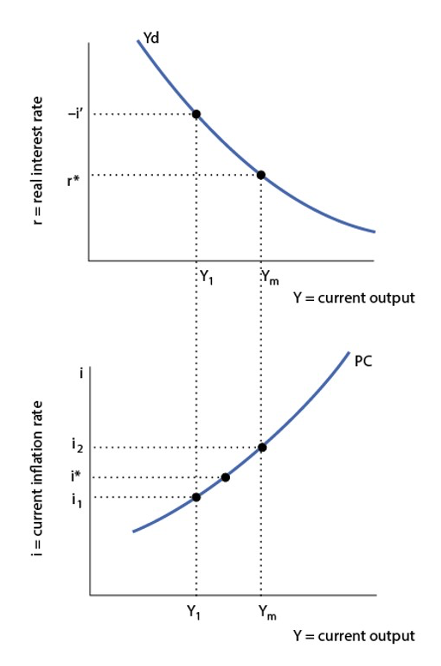
\includegraphics[scale=0.5]{Figures/W_Fig_15pt6.png}
\end{figure}
Now, we have ``too low" inflation and an output gap (want $R$ lower but can't!)
\end{frame}


\begin{frame}
\frametitle[alignment=center]{How can we solve?}
\begin{itemize}
\item Issue:  we want to lower $R$ but can't, it's zero!
\bigskip
\item One possibility: \textbf{forward guidance}
\bigskip
\item Recall that: $i=a(Y-Y_m)+bi'$
\bigskip
\item But of course, $i'=a(Y'-Y_m')+bi''$ tomorrow
\bigskip
\item So we can raise $i$ (lower $r$) even further by promising higher inflation not only today but tomorrow too
\end{itemize}
\end{frame}



\begin{frame}
\frametitle[alignment=center]{Forward Guidance \& Liquidity Trap at the ZLB}
\begin{figure}
\centering
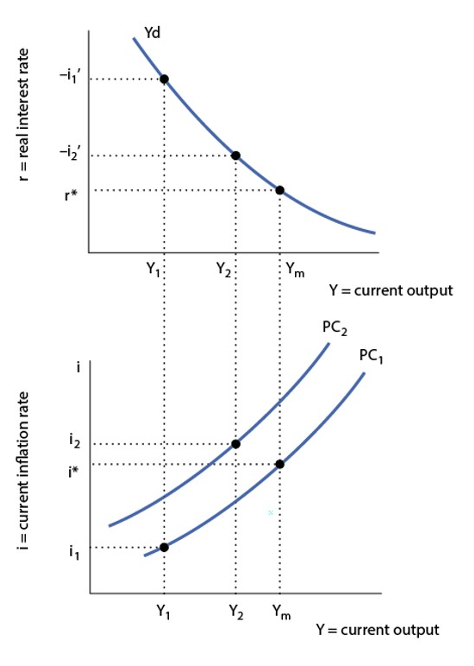
\includegraphics[scale=0.5]{Figures/W_Fig_15pt7.png}
\end{figure}
\end{frame}



\begin{frame}
\frametitle[alignment=center]{The boy who cried wolf}
\begin{itemize}
\item We can lower $r$ now by raising $i$, which we raise by raising $i'$ in future
\bigskip
\item But in future, it may not be in our interest to have higher inflation
\bigskip
\item Commitment dilemma: central bank has to commit to do something that, if it works as intended, it won't want to do
\bigskip
\item Same as studying: writing hard exams is hard, grading them is hard, but I want you to learn
\bigskip
\item If I could tell you the final exam is hard, then you study, learn the material, and everyone better off if I don't write hard exam
\bigskip
\item But, knowing that, you shouldn't study hard
\bigskip
\item Having an institution that values its credibility allows you to avoid this problem (just like being a trustworthy person
\end{itemize}
\end{frame}


\begin{frame}
\frametitle[alignment=center]{Reputation (Tom Sargent)}
\begin{quote}
 In the future, you too will respond to incentives. That is why there are
some promises that you'd like to make but can't. No one will believe those
promises because they know that later it will not be in your interest to
deliver. The lesson here is this: before you make a promise, think about
whether you will want to keep it if and when your circumstances change.
This is how you earn a reputation.
\end{quote}
Q: can you ever promise to do something it isn't in your interest to do? (No, if you include future reputation!)
\end{frame}

\begin{frame}
\frametitle[alignment=center]{Forward Guidance in Practice-Dec. 2008}
\begin{quote}
The Federal Reserve will employ all available tools to promote the resumption of sustainable economic growth and to preserve price stability. In particular, the Committee anticipates that weak economic conditions are likely to warrant exceptionally low levels of the federal funds rate for some time.
\end{quote}
\end{frame}

\begin{frame}
\frametitle[alignment=center]{Forward Guidance in Practice-Dec. 2012}
\footnotesize
\begin{quote}
 … the Committee decided to keep the target range for the federal funds rate at 0 to 1/4 percent and currently anticipates that this exceptionally low range for the federal funds rate will be appropriate at least as long as the unemployment rate remains above 6-1/2 percent, inflation between one and two years ahead is projected to be no more than a half percentage point above the Committee’s 2 percent longer-run goal, and longer-term inflation expectations continue to be well anchored. The Committee views these thresholds as consistent with its earlier date-based guidance. In determining how long to maintain a highly accommodative stance of monetary policy, the Committee will also consider other information, including additional measures of labor market conditions, indicators of inflation pressures and inflation expectations, and readings on financial developments. When the Committee decides to begin to remove policy accommodation, it will take a balanced approach consistent with its longer-run goals of maximum employment and inflation of 2 percent.
\end{quote}
\end{frame}


\begin{frame}
\frametitle[alignment=center]{Forward Guidance in Practice-Mar. 2014}
\footnotesize
\begin{quote}
To support continued progress toward maximum employment and price stability, the Committee today reaffirmed its view that a highly accommodative stance of monetary policy remains appropriate. In determining how long to maintain the current 0 to 1/4 percent target range for the federal funds rate, the Committee will assess progress—both realized and expected—toward its objectives of maximum employment and 2 percent inflation. This assessment will take into account a wide range of information, including measures of labor market conditions, indicators of inflation pressures and inflation expectations, and readings on financial developments. The Committee continues to anticipate, based on its assessment of these factors, that it likely will be appropriate to maintain the current target range for the federal funds rate for a considerable time after the asset purchase program ends, especially if projected inflation continues to run below the Committee’s 2 percent longer-run goal, and provided that longer-term inflation expectations remain well anchored.
\end{quote}
\end{frame}

\begin{frame}
\frametitle[alignment=center]{Forward Guidance in Practice}
\footnotesize
\begin{itemize}
\item Fed kept its options open
\bigskip
\item Forward Guidance wasn't super clear
\bigskip
\item But perhaps that's all they could do--only make promises not only that you intend to keep, but that future you will want to keep
\end{itemize}
\end{frame}


\begin{frame}
\frametitle[alignment=center]{Neo-Fisherism}
\footnotesize
\begin{itemize}
\item Neo-Fisherians think we have the model all wrong
\bigskip
\item Disclaimer:  their model makes more sense to me, but I struggle with empirical evidence!
\bigskip
\item Claim: we should \emph{lower} interest rates to fight inflation, rather than raise them as NK says
\bigskip
\item Why? What's the model?
\end{itemize}
\end{frame}

\begin{frame}
\frametitle[alignment=center]{Output Demand}
\footnotesize
\begin{itemize}
\item Let $Y$ be demand for goods today, $Y'$ be demand tomorrow, $1/d$ be how their relationship changes as a function of the real interest rate $R-i'$ and the natural real interest rate $r^*$
\bigskip
$$Y-Y'=-\frac{1}{d}(R-i'-r^*)$$
\item Basic idea is that tradeoff between demand today and demand tomorrow is governed by interest rates and impatience (the natural real interest rate)
\bigskip
\item An equation like this, the ``Euler Equation" pops up in intertemporal macro all the time
\end{itemize}
\end{frame}

\begin{frame}
\frametitle[alignment=center]{Aside: Euler Equation}
\footnotesize
\begin{itemize}
\item For instance, consider a consumer's problem, where $\beta$ is the discount factor (impatience):
$$u(c,c')=\frac{c^{1-\sigma}}{1-\sigma}+\beta\frac{(c')^{1-\sigma}}{1-\sigma}$$
$$s.t. c+\frac{c'}{1+r}=y+\frac{y'}{1+r}$$
\item Taking first order conditions in a Lagrangian framework, we get:
$$c^{-\sigma}=\lambda$$
$$\beta(c')^{-\sigma}=\frac{\lambda}{1+r}$$
\item Or, combining the two:
$$\left(\frac{c}{c'}\right)^{\sigma}=\beta(1+r)$$
\item Taking logs:
$$\log(c)-\log(c')=-\frac{1}{\sigma}\left(\log(\beta)+\log(1+r)\right)$$
\item Which looks like what Williamson wrote down:
$$Y-Y'=-\frac{1}{d}(R-i'-r^*)$$
\end{itemize}
\end{frame}

\begin{frame}
\frametitle[alignment=center]{Output Demand/Euler Equation}
\footnotesize
\begin{itemize}
\item What does the (new, sensible) Euler Equation say?
$$Y-Y'=-\frac{1}{d}(R-i'-r^*)$$
\item People like so smooth (governed by $d$)
\bigskip
\item Consumption tomorrow relative to today rises more as patience ($\beta$) rises (or for Williamson, $r^*$ falls)
\bigskip
\item Consumption tomorrow relative to today rises more as the real interest rate $R-i'$ rises
\end{itemize}
\end{frame}


\begin{frame}
\frametitle[alignment=center]{Simpler Phillips Curve \& Rational Expectations}
\footnotesize
\begin{itemize}
\item We simplify the Phillips curve to say that inflation is positively related to the output gap (we ignore future inflation, because it won't actually qualitatively affect our results, but makes math harder)
$$i=a(Y-Y_m)$$
\bigskip
\item If $Y_m$ isn't changing, and $r^*$ is also exogenous, we have:
$$i'=a(Y'-Y_m)$$
\item Subsituting in for $Y$ and $Y'$, we get:
$$i'=\frac{a(R-r^*)}{a+d}+\frac{di}{a+d}$$
\item This determines inflation, given an initial value $i_0$.
\bigskip
\item I think a better equation is:
$$\Delta i =-\frac{a}{d}\left(r-r^*\right)$$
\bigskip
\item But both say that $R$ is constant, then inflation will converge to some level
\end{itemize}
\end{frame}

\begin{frame}
\frametitle[alignment=center]{New Keynesian Rational Expectations Model}
\begin{figure}
\centering
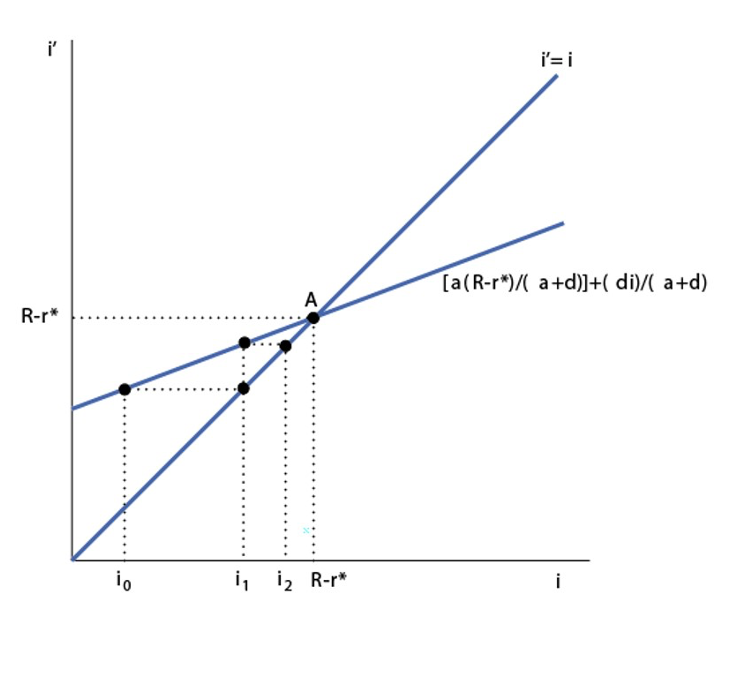
\includegraphics[scale=0.5]{Figures/W_Fig_15pt8.png}
\end{figure}
 Point $A$ is the steady state inflation level
\end{frame}


\begin{frame}
\frametitle[alignment=center]{Long-Run Equilibrium}
\begin{itemize}
\item What is long-run inflation? $i=i'$
$$i'=\frac{a(R-r^*)}{a+d}+\frac{di}{a+d}$$
\item Turns to:
$$i=\frac{a(R-r^*)}{a+d}+\frac{di}{a+d}$$
\item Solving:
$$i=R-r^*$$
\item The long run Fisher equation!  
\bigskip
\item Here, the Fisher effect is \emph{causal}: the long-run inflation rate will be the nominal interest rate minus the real equilibrium interest rate
\bigskip
\item The sense is that if $r^*$ is tied down by human impatience, then given an inflation rate we know what $R$ must be, or given $R$ inflation must be the difference between $R$ and $r^*$.
\bigskip
\item Higher interest rates mean higher inflation!
\end{itemize}
\end{frame}

\begin{frame}
\frametitle[alignment=center]{Short-Run Equilibrium}
\begin{itemize}
\item What happens when we change $R$?
\bigskip
\item Inflation starts to rise, and eventually plateaus until $i=R-r^*$, with the new higher $R$
\bigskip
\item Even in short run, $R$ leads to higher $i$ (contrary to much of what we ``know"!)
\end{itemize}
\end{frame}


\begin{frame}
\frametitle[alignment=center]{Taylor Rule Problems?}
\begin{itemize}
\item How does the Taylor rule do in our new-ish model?
\bigskip
\item Nominal interest rates, bounded at zero, take the form:
$$R=max\left(0,hi+(1-h)i^*+r^*\right)$$
\item Idea:  for now, forget output gap, just look at inflation
\bigskip
\item Higher R when inflation is higher, lower when target $i^*$ is higher, and higher when natural real interest rate $r^*$ is higher
\bigskip
\item We get, when $h>1$ (the recommendation):
$$\begin{cases} R=0 & \text{if }i\leq\frac{h-1}{h}i^*-\frac{r^*}{h} \\ hi+(1-h)i^*+r^* & \text{if }i\geq\frac{h-1}{h}i^*-\frac{r^*}{h}\end{cases}$$
\item Let's draw it!
\end{itemize}
\end{frame}

\begin{frame}
\frametitle[alignment=center]{Our version of the Taylor Rule with ZLB}
\begin{figure}
\centering
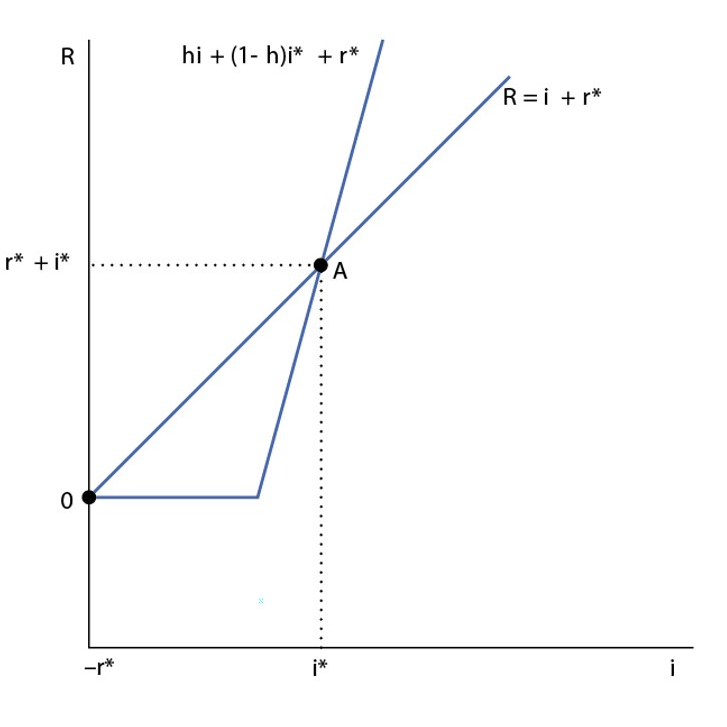
\includegraphics[scale=0.5]{Figures/W_Fig_15pt11.png}
\end{figure}
Euler equation/Output demand+Taylor has two equilibria!
\end{frame}

\begin{frame}
\frametitle[alignment=center]{Exploring Further}
\begin{itemize}
\item Now, take Taylor Rule and apply to Phillips Curve
$$i=max\left(\frac{ar^*}{a+d}+\frac{di}{a+d},\frac{(ah+d)i}{a+d}+\frac{a(1-h)i^*}{a+d}\right)$$
\item We have piecewise linear (kinked) relationship between $i$ and $i'$, let's graph
\end{itemize}
\end{frame}

\begin{frame}
\frametitle[alignment=center]{Our version of the Taylor Rule with ZLB}
\begin{figure}
\centering
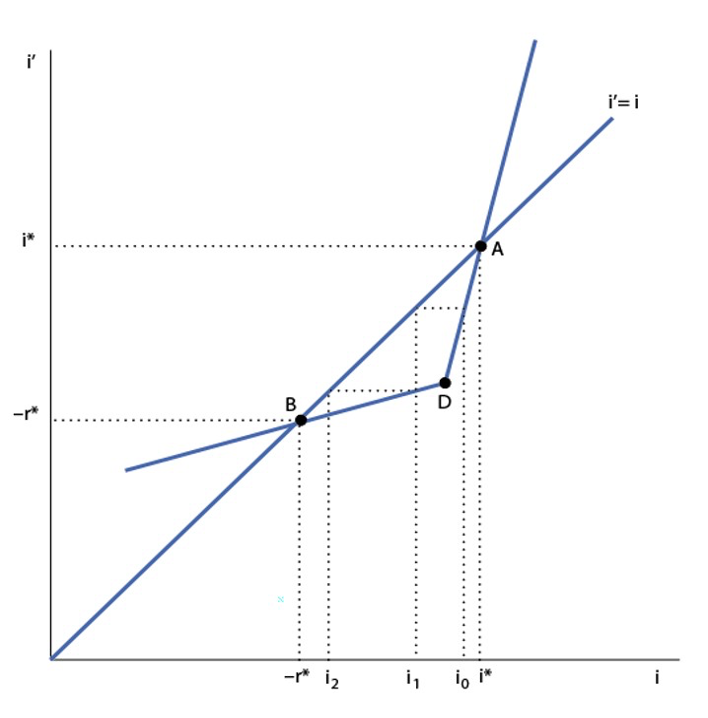
\includegraphics[scale=0.5]{Figures/W_Fig_15pt12.png}
\end{figure}
Euler equation/Output demand+Taylor has two equilibria! $i$ above $d$ converges to positive inflation, $i$ below $d$ converges to zero.
\end{frame}

\begin{frame}
\frametitle[alignment=center]{Basic Idea/Logic}
\begin{itemize}
\item Taylor rule says to react to higher inflation by increasing $R$, lower inflation by decreasing $R$
\bigskip
\item  Fisher effect in NKRE says higher $R$ gives higher inflation, lower $R$ gives lower inflation
\bigskip
\item So if low, then lower $R$ (Taylor rule) then lower inflation (Fisher effect), then lower $R$....
\bigskip
\item And if high, then higher $R$ (Taylor rule) then higher inflation (Fisher effect), then higher $R$....
\bigskip
\item Multiple equilibria!
\bigskip
\item This problem with the Fisher effect isn't just the NKRE model, it's basically everything with an Euler Equation!
\end{itemize}
\end{frame}

\begin{frame}
\frametitle[alignment=center]{Solving the Problem}
\begin{itemize}
\item Instead, could just increase $R$ when inflation needs to be higher
\bigskip
\item We could instead choose to raise $R$ when we want higher inflation, and lower it when current inflation is too high (flip of Taylor)
\bigskip
$$R = \begin{cases}r^*+\frac{(a+d)i^*}{a}-\frac{d}{a}i & \text{ if $i< i^*$} \\
r^*-\frac{d}{a}i^*+\frac{(a+d)i^*}{a} & \text{ if $i\geq i^*$}
\end{cases}$$
\item When we do this, we get what we want, in both cases above, $i'=i^*$
\end{itemize}
\end{frame}

\begin{frame}
\frametitle[alignment=center]{Inflation Under a Neo-Fisherian Monetary Policy Rule}
\begin{figure}
\centering
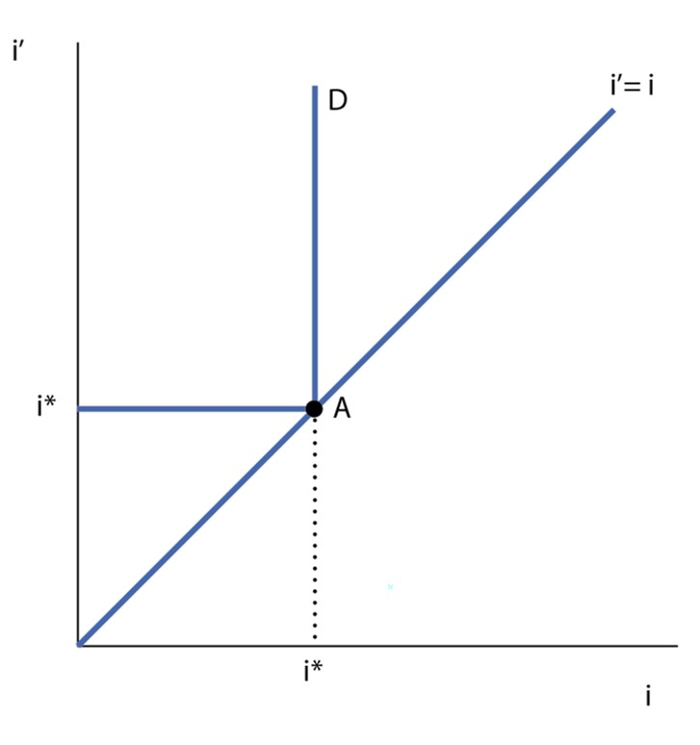
\includegraphics[scale=0.5]{Figures/W_Fig_15pt13.png}
\end{figure}
\end{frame}

\begin{frame}
\frametitle[alignment=center]{Idea}
\begin{itemize}
\item Euler equation/output demand relates output today and tomorrow with nominal interest rates, inflation, and human impatence (``natural real rate)
\bigskip
\item Phillips curve relates output demand today and tomorrow with inflation today and tomorrow
\bigskip
\item Combining, we get that the change in inflation relates to nominal interest rates (-) and human impatience (+)
\bigskip
\item If inflation too low, raise nominal interest rate, which increases inflation tomorrow relative to today (moves us toward right path)
\bigskip
\item Lower nominal interest rates lowers consumption (output) growth, which lowers inflation tomorrow
\bigskip
\item Higher nominal interest rates increase consumption (output) growth, raising inflation tomorrow 
\end{itemize}
\end{frame}

\begin{frame}
\frametitle[alignment=center]{My own take}
\begin{itemize}
\item This model makes sense!
\bigskip
\item I ``want" to be a Neo-Fisherian
\bigskip
\item But some stories hold me back: ``Volcker Shock" 
\bigskip
\item Claim: Paul Volcker came into office in October 1979, and changed policy, dramatically increased nominal interest rates, and inflation fell
\bigskip
\item Treated as similar to a ``natural experiment"
\end{itemize}
\end{frame}

\begin{frame}
\frametitle[alignment=center]{Volcker Shock}
\begin{figure}
\centering
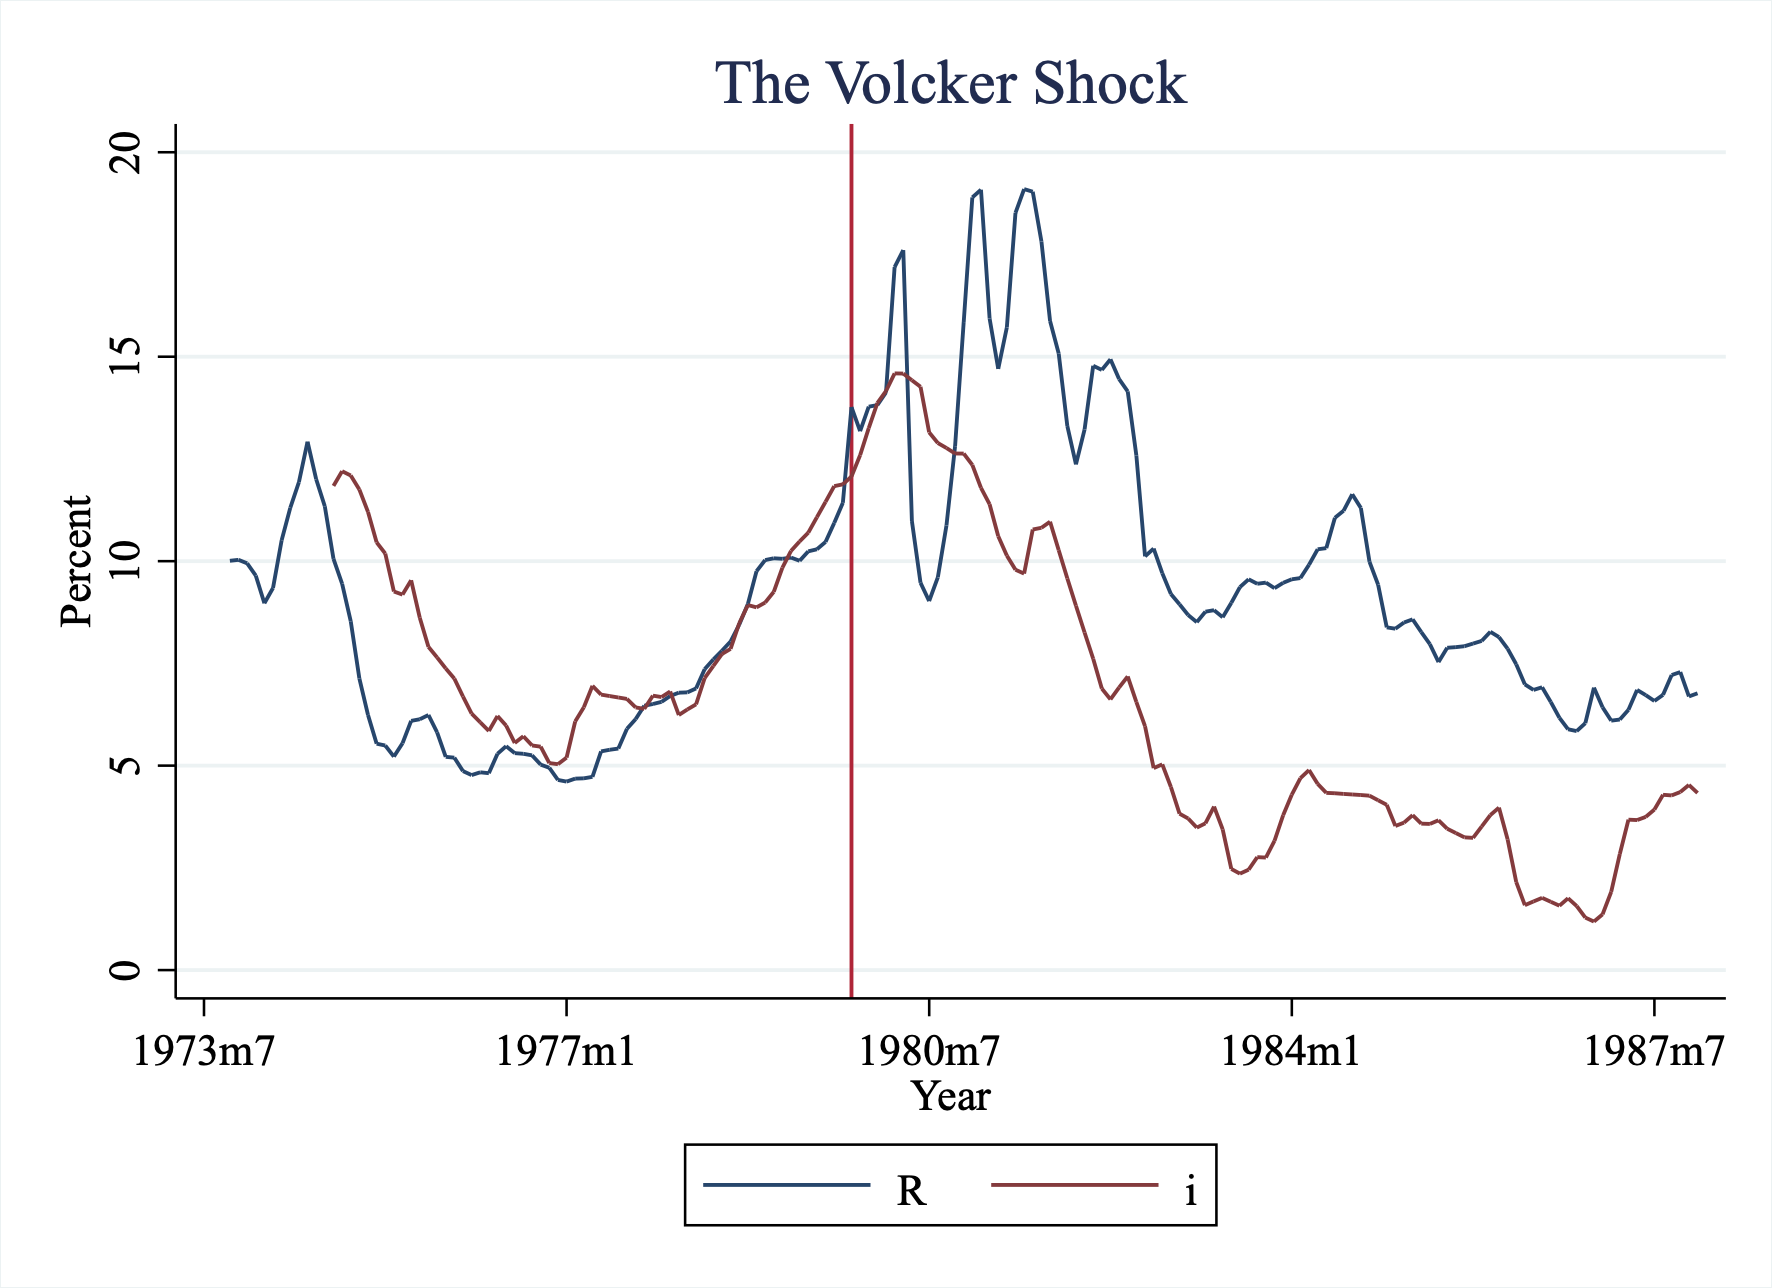
\includegraphics[scale=0.35]{Figures/VolckerShock.png}
\end{figure}
\end{frame}

\begin{frame}
\frametitle[alignment=center]{But Neo-Fisherians have something to work with!}
\begin{figure}
\centering
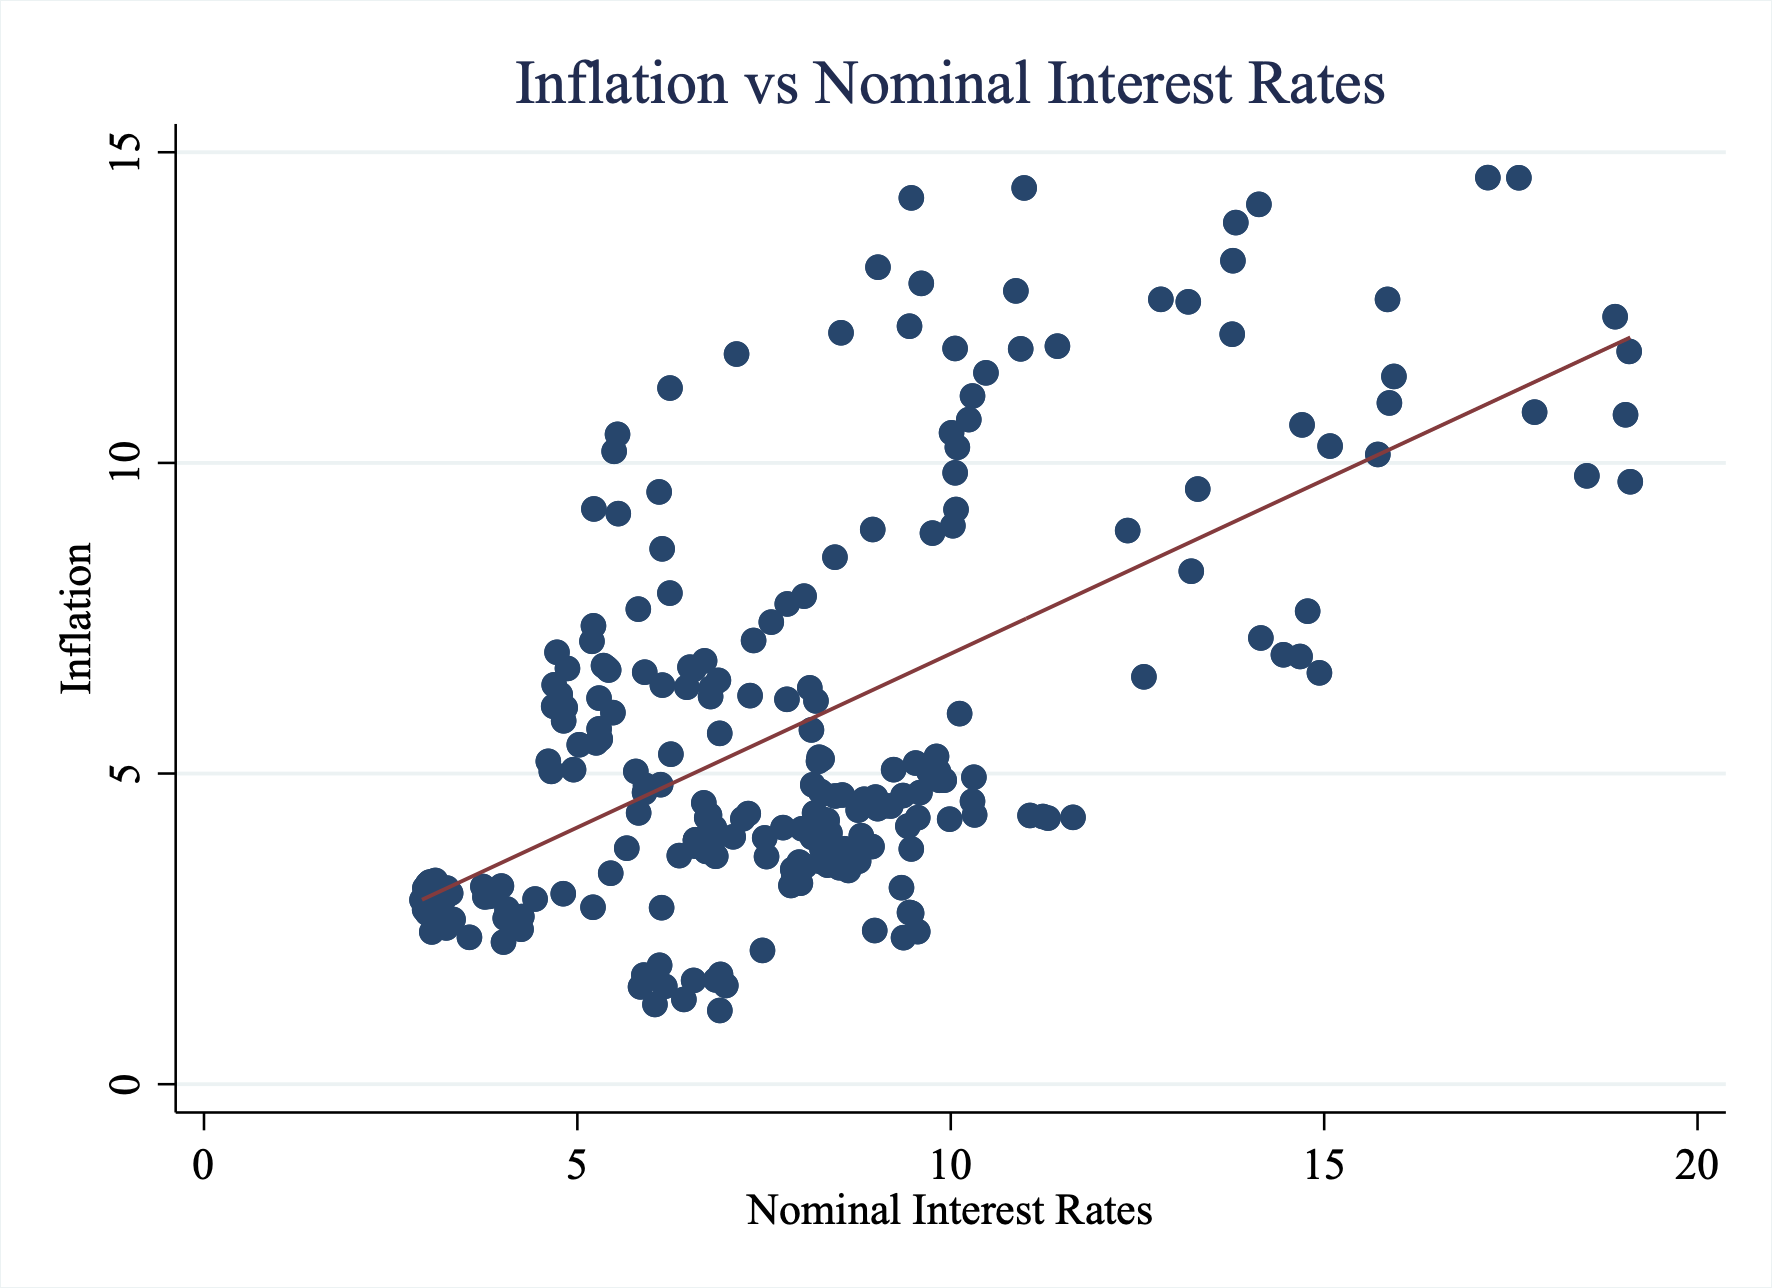
\includegraphics[scale=0.33]{Figures/NeoFisher.png}
\end{figure}
\end{frame}

\begin{frame}
\frametitle[alignment=center]{Conclusions}
\begin{itemize}
\item Even the NK model has some wrinkles
\bigskip
\item Subtle wrinkles can totally upend even the \emph{direction} of policy advice!
\bigskip
\item Currently these Neo-Fisherian theories are not commonly accepted
\bigskip
\item But as I say, they keep me up at night
\bigskip
\item Next we turn to open economy macro: trade, etc.!
\end{itemize}
\end{frame}


\end{document}